\documentclass{article}
    \usepackage[utf8]{inputenc}
    \usepackage[T1]{fontenc}
    \usepackage{lmodern}
    \usepackage{amsmath}
    \usepackage{amssymb}
    \usepackage{mathrsfs}
    \usepackage{tikz}
    \usepackage{graphicx}
    \usepackage{placeins}
    \usepackage{listings}
    \usepackage{cancel}
    \usepackage{hyperref}
    \usepackage{subcaption}
    \usepackage{xcolor}
    \colorlet{punct}{red!60!black}
    \definecolor{background}{HTML}{EEEEEE}
    \definecolor{delim}{RGB}{20,105,176}
    \colorlet{numb}{magenta!60!black}
    
    \newcommand{\deriv}{\mathrm{d}}
    \usepackage{array,multirow,makecell}
    \usepackage[top=2cm, bottom=3cm, left=2cm,right=2cm]{geometry}
    \usepackage{bbold}
    \newtheorem{problem}{Problem}
    \newtheorem{definition}{Definition}
    \newtheorem{conjecture}{Conjecture}
    \newtheorem{lemma}{Lemme}
    
    \usepackage{fancyhdr}
    \pagestyle{fancy}
    \fancyhead[L]{Marc-Antoine \bsc{Augé} - Team J5}
    \fancyhead[C]{Final Submission - Abstract}
    \fancyhead[R]{Challenge ROADEF}
    \renewcommand{\headrulewidth}{1pt}
    \fancyfoot[C]{\thepage}
    
    \newcolumntype{C}[1]{>{\centering\arraybackslash }b{#1}}
    \setcounter{MaxMatrixCols}{20}
    \renewcommand{\footrulewidth}{1pt}
    
    \title{ROADEF / EURO Challenge 2018 \\
    - Final Submission-}
    \date{January 23th, 2019}
    \author{Marc-Antoine \bsc{Augé} (Team J5)}
    
    \begin{document}
        \maketitle

\paragraph{Abstract}
The participation of the team J5 is simply a constructive algorithm which was improved month after month. It mixes a deep understanding of the problem and lot of computer engineering to compute every step fast. This algorithm finds some best known solutions (on instances A1, A17 and A20) with an average occupation rate greater than $81\%$ on instances A and B. In view of all the progress made between the sprint phase, the qualification phase and the final one, it sure that better results could be found in the future.

\section{Introduction}

The optimization algorithm described rests on two algorithms: one generates the order of items wanted at the output and the other builds a cutting pattern corresponding to this sequence. The first algorithm is simply a localsearch on this sequence. As the second algorithm is called at every sequence generated, it has to be both as fast as possible and as good as possible. It's a greedy-constructive algorithm based on complex structures with lot of computer engineering.

\section{The LocalSearch}

As the goal of this algorithm is to browse only possible sequences, the sequences set is modelized as follow:

\begin{definition}[Notations]
    Let $H$ the height of a plate and $W$ its width. 
    Let $K$ the number of stacks. 
    Let $N$ the number of items.
\end{definition}

\begin{definition}[A Sequence]
    Let $n_k$, $k \in [|0, K - 1|]$ the number of items in the stack $k$.\\
    A \textit{sequence} is defined as a permutation of the sequence:
\begin{center}0,..,0 ($n_0$ times), ..., k, ..., k ($n_k$ times), ..., K, .., K ($n_K$ times)\end{center}

    It corresponds to the sequence of stacks called. For example if the instance has three stacks $s_0 -> [0, 1, 2]$ (stack 0 contains three elements, 0 then 1 then 2), $s_1 -> [3] $ and $s_2 -> [4, 5]$, then:
    \begin{itemize}
        \item The sequence \textit{0, 0, 1, 2, 0, 2} means \textit{item 0, item 1, item 3, item 4, item 2, item 5}.
        \item The sequence \textit{0, 1, 2, 2, 0, 0} means \textit{item 0, item 3, item 4, item 5, item 1, item 2}
    \end{itemize}
\end{definition}

With this notation, every sequence is feasible (if there are enough plates available, we can always put one item per plate).

\subsection{Moves}

The moves used in this LocalSearch are basic: 
\begin{itemize}
    \item \textbf{Swap}: it swaps two elements in the sequence ;
    \item \textbf{K-Successive Permutation}: it shuffles K consecutive elements ($K$ between 3 and 7) ;
    \item \textbf{K-Permutation}: it shuffles K random elements ($K$ between 3 and 5) ;
    \item \textbf{K-Insert}: it moves a block of K elements along the sequence ($K$ between 1 and 3)
\end{itemize}
If a move changes the same stacks (for example, if there is only one stack), it is not tested. Therefore they are 10 moves and they are equaly likely. If a move doesn't change the sequence, the second algorithm is not called.

\subsection{Objectives}

The LocalSearch main objective is the surface occupation but LocalSearch also have lexicographic objectives: the surface occupation of every plate. These objectives are prioritized from the first plate to the last one.
It means that if two solutions have the same score, the better is the solution with the highest occupation ratio for the first plate, and if equals, for the second plate etc. Two solutions are equals if and only if the score and the surface occupations are the same. A move is accepted if it improves the solution.

\section{The Constructive Algorithm}

    \subsection{The problem}
This algorithm takes as input the output sequence of item. Its goal is to build the better solution possible which respects this sequence.

Let $N$ the number of items and $(i_0, ..., i_N)$ the input sequence\footnote{Even if the LocalSearch works on \textit{stacks sequence}, it gives to the Constructive Algoritme an \textit{items sequence}.}. 
A cutting pattern is modelized as a sequence of \textit{Locations} where a \textit{Location} is simply an item, coordinates ($x$, $y$ and a bin index) and a boolean variable which means if the item is rotated or not.

\begin{definition}[Location]
Let $L$ a location, we denote $(L_x, L_y)$ the coordinates of the lower-left corner, $(L_{xw}, L_{yh})$ the coordinates of the top-right corner.
\end{definition}

\begin{problem}[Constructive Algorithm Problem]
Given an input items sequence $(i_0, ..., i_N)$, find the locations sequence $(L_0, ..., L_n)$ minimizing the surface occupation and respecting all the constraints.
\end{problem}

To obtain this locations sequence, the algorithm is constructive and finds locations one after another. It builds the locations from the first bin to the last one and only need infos on the locations in the current bin.

\begin{problem}
Let $0 \leq k  < N - 1$, let $(L_0, ..., L_k)$ a locations sequence who respects all the constraints (except cutting all items).

Find $L_{k + 1}$ a location such as $(L_0, ..., L_{k + 1})$ is feasible (and as good as possible).
\end{problem}

    \subsection{Theory}
    Let $0 \leq k  < N - 1$, let $(L_0, ..., L_k)$ a locations sequence who respects all the constraints (except cutting all items). Without loss of  generality, suppose that all locations are on the same bin.

    In the two next sections (about The Green Star and The Red Monster), defects are ignored.

        \subsubsection{The Green Star}

The Green Star is a complex structure introduced to transpose into the problem the idea that between two locations at the same $y$, the one with the lower $x$ is better (same by permutating $x$ and $y$) than the other. This idea is wrong in the whole problem if we consider the constraints on the cutting pattern but remains a good heuristic.

\begin{definition}[The Green Star]
    The Green Star of $(L_0, ..., L_k)$ is defined by $ (x, y) \in [|0, W|]\times[|0, H|]$ such as there exists $i, j \leq k$ such that $x \leq s^i_{xw}$ and $y \leq s^j_{yh}$.
\end{definition}

\begin{conjecture}[The Green Star Condition]
    Every $L_{k + 1}$ must be out of the Green Star of $(L_0, ..., L_k)$ to be feasible.
\end{conjecture}

The best locations according to the Green Star are the blue points in Figure \ref{fig:gull}: each one is feasible (expecting constraints about the trees like the depth, the trimming, the minwaste...) and every other location is less good.

The implementation of Green Star only needs the list of points which are in its border, other points can be forgotten. The implementation gives the following complexities, if $p$ is the number of points at its border (in practive $p < 5$).

\begin{itemize}
    \item Add a new point can be is at worst in $O(p)$ (it's possible to sort the points by x to be more efficient).
    \item Find all solutions possible in $O(p)$.
\end{itemize}

The Green Star, with the defects management and the tree checker/builder and with a little greedy algorithm can find feasible solutions with a surface occupation ratio of $72\%$. It was the algorithm used for the sprint phase.

        \subsubsection{The Red Monster}
As the \textit{Green Star Algorithm} does not find the optimum of instance \textit{A1}, the Red Monster is the correction of the Green Star to keep optima locations. It is much more complex than the Green Star, since the Red Monster memorizes when each item must be cut, in order to remove unfeasable locations due to the cutting order.
The figure 1.b shows the differences between both structures and how the Red Monster is able to accept the optima of A1, unlike the Green Star.

\begin{figure}
    \centering
    \begin{subfigure}[b]{0.48\textwidth}
        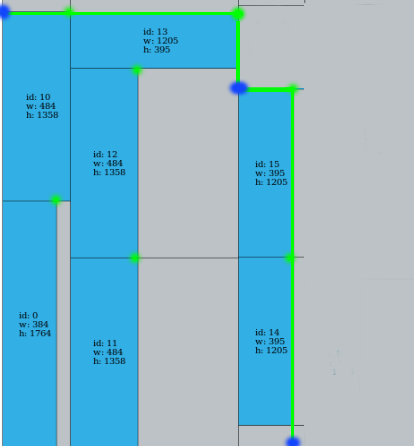
\includegraphics[height=7cm]{greenStart.png}
        \caption{The Green Star defines the few possible locations (blue points) which cannot be easily improved.}
        \label{fig:gull}
    \end{subfigure}
    ~ %add desired spacing between images, e. g. ~, \quad, \qquad, \hfill etc. 
      %(or a blank line to force the subfigure onto a new line)
    \begin{subfigure}[b]{0.48\textwidth}
        \centering
        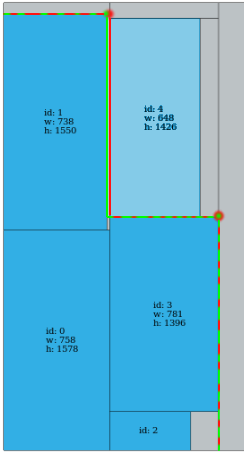
\includegraphics[height=7cm]{greenvsred.png}
        \caption{The Green Star VS the Red Monster : the Green Star tries a location more in the left that the Red Monster and therefore ignores the optima.}
        \label{fig:tiger}
    \end{subfigure}
    ~ %add desired spacing between images, e. g. ~, \quad, \qquad, \hfill etc. 
    %(or a blank line to force the subfigure onto a new line)
    \caption{Structures discovered and used}\label{fig:animals}
\end{figure}

        \subsubsection{Defects Management}
The idea to manage defects is to find a Location without looking at them (with the Red Monster Algorithm) and then see if it contains defects. If not, the location is correct. If the location contains defects, the Defects Mananager Algorithm moves the location (increases $x$ and $y$) in order to find all feasible locations. It keeps only \textit{best locations} in the way that if two locations have the same $x$, the location with the lower $y$ is better.

        \subsubsection{Cutting Pattern Checker and Builder}
Because the Red Monster Algorithm is not able to find locations which are respecting all the constraints »trimming for example), another algorithm try to build a correct tree cutting pattern from $(L_0, ..., L_{k + 1})$. The location $L_{k + 1}$ is feasible if and only if a tree cutting pattern can be build.

To build this cutting pattern, the idea is to look at all the cuts which may be possible, they are the extremities of each item. Then the algorithm determines for each if it's really possible (does this cut go through an item? does this cut break the requested output sequence?) and made the cuts. This algorithm is called recursively on each node created.

Many improvements have been made on this algorithm because it's the slowest algorithm of the software. For example, as the algorithm is mainly needed to check if the last location is feasible, it works better if the cuts are made from right to left (if it fails, it fails sooner).

    \subsection{Practice}
        \subsubsection{DeepScore algorithm}
The Constructive Algorithm have to find a way to find the best location among all of them given by the Red Monster Algorithm. To do this, the idea is to have a greedy algorithm with a backtracking. It means that to find the better location, it tests all the locations possible and all their descendants for many generations (3 to 4 generations in practice) and takes the best one.

\subsubsection{Improvements}
    \paragraph{Don't compute useless unmodified bins}
As the items sequence in input does not change a lot, many bins are unmodified. For example all the bins before the bin which contains the first item position modified. They are not computed another time.

Some bins at the end are also unmodified but their detection is hard and the implementation tested is slower than building them each time.

    \paragraph{Pruning less good solutions}
If a location abscissa is after the best abscissa found (total surface occupation), it's less good so the location is automaticaly refused. This could be improved with better bounds on the problem but it's complicated to do that quick.

    \paragraph{Storing the search tree}
The search tree is computed many times because it's computed on 4 generations to find the best location for first item, then to find the best location for second item... Therefore, the tree can be saved. Now, the tree has only need to be a little bit enlarged to find the second best location etc.

    \paragraph{Use our algorithm as bound}
The search tree can be really: if each node have height children,  they are 4680 nodes to checked (by calling the check / tree builder). As the Red Monster algorithm is really fast, it can build this tree fast but it's slow to build the tree. Therefore the idea is to build the tree once without using the Tree Checker and after that read this tree, look first to the good locations without tree checking and stop once a correct location is find. By doing this, much less locations are checked than before.

\section{Results}

Our results were obtained on a computer with \textbf{Intel(R) Core(TM) i7-3537U CPU @ 2.00GHz} (2 Cores) in 180 seconds and with height threads (as is the same configuration as for the evaluation). No computations in 3600s.\\
We obtained an average value of \textbf{84,4\%} on instances A, \textbf{78,3\%} on instances B and \textbf{81\%} on instances A and B.
    \end{document}
    